\section{Introduction} % Pas de numérotation
\addcontentsline{toc}{section}{Présentation du sujet} % Ajout dans la table des matières

\subsection{A brief presentation of the project}

\paragraph{}

There are lots of applications on the Internet to help people improve their english. But we wanted to do it in a really pedagogically way, so that the learner wouldn't give up after a few weeks. Therefore, to motivate him and motivate him to learn without being bored, we created a website designed to teach "student" users with interesting stories. \linebreak
You can access the website through this URL: \textbf{\emph{\url{http://1.anglofun-1291.appspot.com}}} \linebreak

\begin{figure}[!ht]
    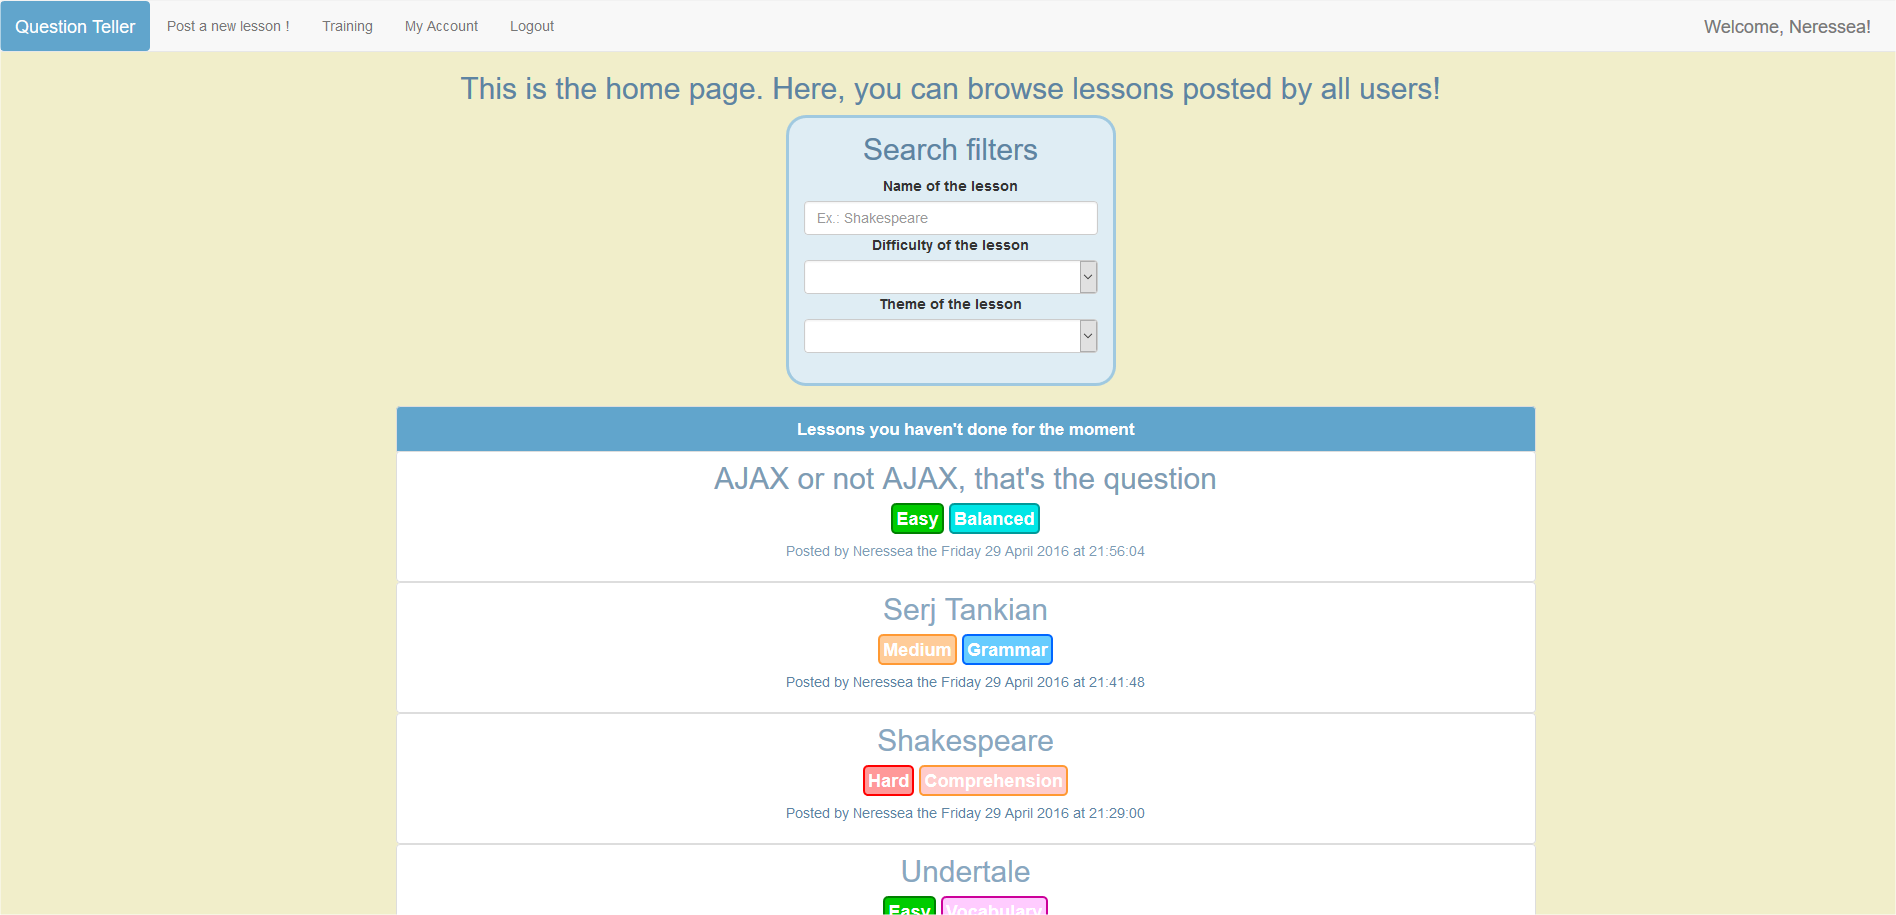
\includegraphics[width=0.5\textwidth]{./images/snapshot1.png}
    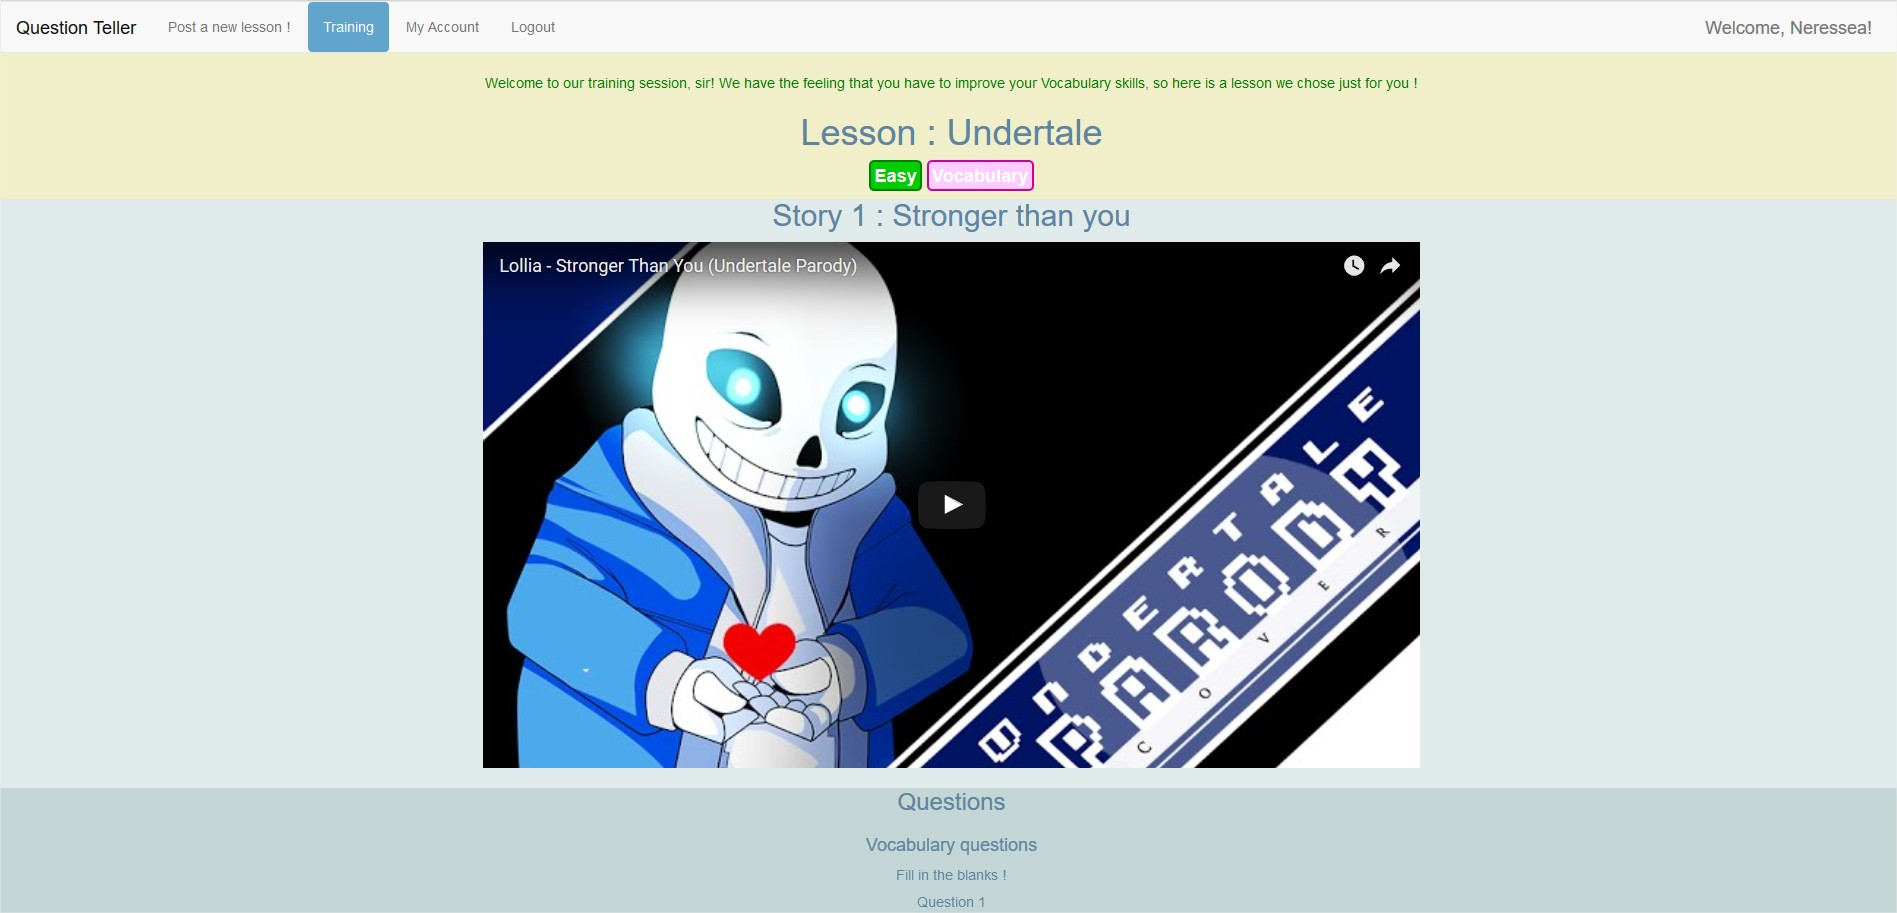
\includegraphics[width=0.5\textwidth]{./images/snapshot2.jpg}
    \caption{Snapshots of the website}
\end{figure}

\subsection{Specifications}

\paragraph{}
Thus, our objectives were to allow users to try lessons to improve themselves, each lesson being composed by several stories and questions related to it. But we didn't want to create a huge and static database of stories from the beginning. We thought it would be more entertaining if all users could create their own stories and send it to other users. But that's not all. The main feature of our application is certainly the "Training program" proposed by the server, in which the website trains the user by sending him adapted lessons.
To perform the best user experience, we also wanted the website to be responsive, so the user can either use it on a computer or a tablet. 


\paragraph{}
Now, we will see in details these different features and after that we will present you their technical side.
